% 原书 p.34–p.38（PDF p.42–p.46）
% >>> p042
\section{群作用（Group Action）}

\begin{keytakeaways}
\begin{itemize}
  \item 物理图像：物理系统的对称性由群 $G$ 在相空间上的作用实现；连续对称性对应
        Lie 群，其无穷小生成元是 Lie 代数 $\mathfrak{g}$ 中的向量。
  \item 数学工具：Lie 群与 Lie 代数、左不变向量场 $X^v$、指数映射 $\exp$、
        Lie 代数同态 $\varphi:\mathfrak{g}\to C^\infty(M)$，以及辛作用与哈密顿作用的
        两个条件 (i)(ii)。
  \item 几何观点：辛作用只要求 $\mathcal{L}_{X_v}\omega=0$（即 $\iota_{X_v}\omega$ 闭）；
        哈密顿作用进一步要求 $\iota_{X_v}\omega$ 恰当，且 $v\mapsto H_v$ 保持括号。
  \item 本节结论：有效 $\T^n$-作用给出迷向轨道，从而 $\dim M\ge2n$（例 2.4.3）；
        $SO(3)$ 在 $T^*\R^3$ 上的作用给出角动量 $\mu(q,p)=q\times p$ 的雏形（2.26），
        为 §2.5 的矩映射作准备。
\end{itemize}
\end{keytakeaways}

辛流形上构造的许多不变量，若在某种意义上具有对称性，往往变得相当容易计算。受经典物理中
由群作用给出的对称性的启发，有一大类辛流形容许群作用。为了精确地描述它们，我们先回顾
Lie 群论的一些背景知识。

回顾：若群 $G$ 还配有与群乘法相容的流形结构，则称 $G$ 为 \textbf{Lie 群}（Lie group）。
对每个 Lie 群 $G$，可联系一个 \textbf{Lie 代数}（Lie algebra）$\mathfrak{g}$，其定义为
$G$ 在单位元 $e$ 处的切空间，即 $\mathfrak{g}=T_eG$。

注意，只研究 Lie 群在单位元 $e$ 处的切空间便足够了，因为任何切向量
$v\in T_eG=\mathfrak{g}$ 都可被转移到流形上任意其他点的切空间中——只需用群 $G$ 的
（左）乘法所诱导的微分去推前即可。通常用 $L_g$ 记此乘法，并用 $\dd L_g$（$g\in G$）记
诱导的微分。因此，对任意向量 $v\in\mathfrak{g}$，我们可把它延拓为向量场 $X^v$
（称为\textbf{由 $v$ 生成的左不变向量场}），定义如下
\begin{equation}
  X^v(g):=(\dd L_g)_e(v)\qquad\text{对任意 } g\in G .
  \tag{2.18}
\end{equation}
% [Tutor Note: 这里 $L_g:G\to G$ 是左乘映射 $h\mapsto gh$，故
% $(\dd L_g)_e:T_eG\to T_gG$。注意 (2.18) 用 $L_g$ 而非右乘；若改用右乘，得到的将是
% 右不变向量场，其 Lie 括号相差一个符号。$X^v$ 的左不变性指
% $(\dd L_g)_hX^v(h)=X^v(gh)$，据此可验证 $[X^v,X^w]$ 仍左不变，这是下方 Lie 括号
% 良定义的关键。]

这有助于我们如下定义 $\mathfrak{g}$ 上的（代数）\textbf{Lie 括号}
\[
  [v,w]:=\big([X^v,X^w]\big)(e),
\]
其中 $X^v,X^w$ 分别是由 $v,w\in\mathfrak{g}$ 生成的左不变向量场。

下面我们列出 Lie 群的一些基本例子。更多细节见 [145] 第 7 章。

\begin{wexam}{2.4.1}
若 $G=\R^n$，则 Lie 代数为 $\mathfrak{g}=\R^n$。对任意向量 $v\in\mathfrak{g}$，在
$\mathfrak{g}=T_0\R^n$ 的标准基 $\{e_1,\cdots,e_n\}$ 下（事实上这组基适用于任意切空间
$T_g\R^n$），有 $v=(v_1,\cdots,v_n)$。平移 $L_g$ 就是移位 $0\mapsto g$，于是对上述 $v$，
对任意 $g\in\R^n$ 有 $\dd L_g(v)=(v_1,\cdots,v_n)\in T_g\R^n$。注意所得的 $\dd L_g(v)$
只依赖于 $v$。因此诱导出的左不变向量场为
\begin{equation}
  X^v=(v_1,\cdots,v_n).
  \tag{2.19}
\end{equation}
于是对任意 $v,w\in\mathfrak{g}$ 都有 $[v,w]=0$（因为对任意基元 $e_i,e_j$ 有
$[e_i,e_j]=0$）。同样的论证对标准环面 $\T^n$ 也成立。\hfill$//$
\end{wexam}

\begin{wexam}{2.4.2}
设 Lie 群 $G$ 是矩阵群 $SO(n)\le GL(n;\R)$。则 Lie 代数 $\mathfrak{g}$ 由 $G$ 中光滑
曲线在单位矩阵处的导数组成。可以验证
$\mathfrak{g}=\{A\in M_{n\times n}(\R)\mid A+A^{\mathrm T}=0\}$。对任意
$v,w\in\mathfrak{g}$，Lie 括号由矩阵换位子给出，即 $[v,w]=v\cdot w-w\cdot v$。
通常 $SO(n)$ 的 Lie 代数记作 $\mathfrak{so}(n)$。\hfill$//$
\end{wexam}

% >>> p043
Lie 群论中另一个重要的定义是把 Lie 群 $G$ 与其 Lie 代数 $\mathfrak{g}$ 联系起来的
指数映射。

\begin{wdefn}{2.4.1}
给定 Lie 群 $G$，\textbf{指数映射}（exponential map）$\exp:\mathfrak{g}\to G$ 定义为
\[
  \exp(v):=\gamma_v(1),
\]
其中 $\gamma_v$ 是 (2.18) 中定义的左不变向量场 $X^v$ 的、以单位元 $e\in G$ 为起点、
以 $v\in\mathfrak{g}$ 为方向的唯一积分曲线。
\end{wdefn}

指数映射是局部微分同胚，并具有如下性质：若 $[v,w]=0$，则
\[
  \exp(v+w)=\exp(v)\cdot\exp(w).
\]
一般地，若 $[v,w]=0$ 不成立，则 $\exp(v+w)$ 的表达式相当复杂。著名的
Baker--Campbell--Hausdorff 公式告诉我们，$\exp(v+w)$ 的展开只能由 $v$ 与 $w$ 的
（高阶或迭代）Lie 括号表出。关于其历史，见 [11]。

对来自矩阵群的 Lie 群，由于 Lie 括号有显式的意义（即换位子）（例如见例 2.4.2），
矩阵指数的通常级数展开为
\begin{equation}
  \exp(v)=\mathbf{1}+v+\frac{v^2}{2!}+\frac{v^3}{3!}+\cdots .
  \tag{2.20}
\end{equation}
% [Tutor Note: 术语依据——exponential map 在此译「指数映射」；它与 Riemann 几何中测地线
% 意义下的指数映射在紧 Lie 群上一致（取双不变度量时），但本书语境只用 Lie 群意义。
% (2.20) 中 $\mathbf{1}$ 是单位矩阵，按本工程约定不用 $\mathbb{1}$。]

现在回到本节开头提出的问题：研究带对称性的辛流形。这里有一个自然的问题。

\begin{wque}{2.4.1}
Lie 群的作用如何与辛结构发生关联？
\end{wque}

给定被 Lie 群 $G$ 作用的辛流形 $(M,\omega)$，对固定点 $x\in M$ 与切向量
$v\in\mathfrak{g}$，作用在 $x$ 上的一族指数映射 $\exp(tv)$ 在 $x$ 附近描出一条曲线
（见图 2.3）。考虑它在 $x$ 处的导数，即
\begin{equation}
  \left.\frac{\dd}{\dd t}\exp(tv)(x)\right|_{t=0}=:X_v(x).
  \tag{2.21}
\end{equation}
% >>> p044
当让 $x$ 跑遍整个 $M$ 时，我们得到一个向量场 $X_v$（于是记号 $X_v(x)$ 正好体现它是
点 $x$ 处的向量场）。这个向量场 $X_v$ 促使我们给出如下定义。

\begin{figure}[htbp]
  \centering
  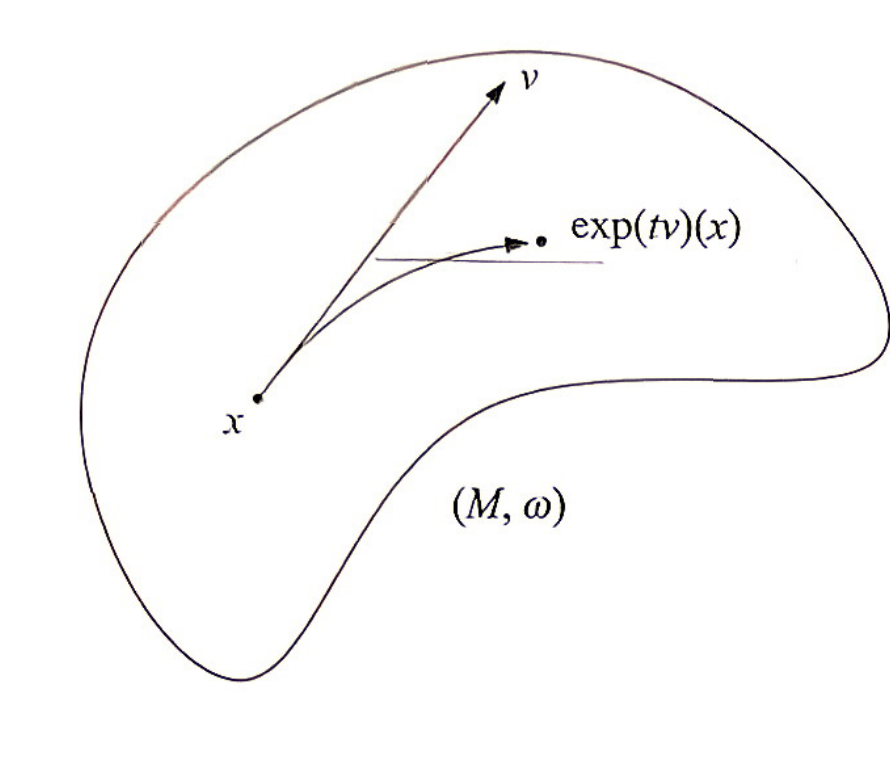
\includegraphics[width=0.56\linewidth]{figures/fig_p044_1.png}
  \caption*{图 2.3\quad $(M,\omega)$ 上的指数映射（原书 p.36, Figure 2.3；PDF p.44）}
\end{figure}

\begin{wdefn}{2.4.2}
给定被 Lie 群 $G$ 作用的辛流形 $(M,\omega)$，若 (2.21) 中构造的向量场 $X_v$ 满足
\begin{equation}
  \mathcal{L}_{X_v}\omega=\dd\iota_{X_v}\omega=0
  \tag{2.22}
\end{equation}
对每个 $v\in\mathfrak{g}$ 成立，则称 $G$ 在 $(M,\omega)$ 上的作用为\textbf{辛群作用}
（symplectic group action）。若对每个 $v\in\mathfrak{g}$，向量场 $X_v$ 进一步满足如下
条件：
\begin{enumerate}[label=(\roman*)]
  \item 存在 $H_v\in C^\infty(M)$ 使得 $\iota_{X_v}\omega=-\dd H_v$（由定义 1.7.1，
        $X_v$ 是由 $H_v$ 生成的哈密顿向量场）；
  \item 由上面的条件 (i) 给出的对应 $\varphi:\mathfrak{g}\to C^\infty(M)$，
        $v\mapsto H_v$，是从 $(\mathfrak{g},[\cdot,\cdot])$ 到
        $(C^\infty(M),\{\cdot,\cdot\})$ 的 Lie 代数同态，即
        \[
          \varphi([v,w])=\{\varphi(v),\varphi(w)\}=\{H_v,H_w\}
          \qquad\text{对任意 } v,w\in\mathfrak{g},
        \]
\end{enumerate}
则称该群作用为\textbf{哈密顿群作用}（Hamiltonian group action）。
\end{wdefn}
% [Tutor Note: (2.22) 用到了 Cartan 公式 $\mathcal{L}_{X}=\dd\iota_X+\iota_X\dd$ 与
% $\dd\omega=0$，故辛作用等价于每个 $\iota_{X_v}\omega$ 是闭 1-形式。这里的「辛作用」
% 只要求 $\omega$ 在流作用下不变（辛同痕），并不要求存在整体 Hamilton 函数；两者之差正是
% 一维 de Rham 上同调 $H^1(M;\R)$ 中的「通量」类（flux）。故 §2.2 的哈密顿同痕只是
% 辛同痕的特例。]

注意定义 2.4.2 中的关系 (2.22) 有清晰的几何意义：向量场 $X_v$ 的流保持辛结构 $\omega$。
换言之，$X_v$ 的流是一个辛同痕，即一族辛同胚（见定义 1.5.1）。由 (2.22) 还可读出辛群
作用的另一种等价说法：形式 $\iota_{X_v}\omega$ 是闭 1-形式（与之相比，对哈密顿群作用，
定义 2.4.2 的 (i) 要求 $\iota_{X_v}\omega$ 是恰当 1-形式）。我们强调，要得到哈密顿群作用，
除 $\iota_{X_v}\omega$ 的恰当性外，还需要定义 2.4.2 中的条件 (ii)。不过条件 (ii) 往往
容易验证。

下面这个例子说明，哈密顿群作用可对辛流形产生拓扑上的限制。

\begin{wexam}{2.4.3}
给定带哈密顿群作用的辛流形 $(M,\omega)$，作用群为环面 $\T^n$。由定义 2.4.2 的条件
(ii)，对任意 $v,w\in\mathfrak{g}=\R^n$，对应 $\varphi:\mathfrak{g}\to C^\infty(M)$
满足
\begin{equation}
  0=\varphi([v,w])=\{\varphi(v),\varphi(w)\}=\{H_v,H_w\}=\omega(X_w,X_v),
  \tag{2.23}
\end{equation}
其中第一个等号来自例 2.4.1 中 $[v,w]=0$ 这一事实，而最后一个等号来自定义 2.3.1 中
泊松括号的定义，再加上定义 2.4.2 条件 (i) 中 $H_v,H_w$ 的定义性质。
% >>> p045
现在假设存在某点 $x\in M$，使得此 $\T^n$-作用在 $x$ 处的稳定化子恰为单位元
$e\in\T^n$，简写为
\begin{equation}
  \T^n_x=\{e\}.
  \tag{2.24}
\end{equation}
于是由轨道–稳定化子定理，有
$\T^n\cdot\{x\}\cong\T^n/\T^n_x=\T^n$。故轨道 $\T^n\cdot\{x\}$ 的维数为 $n$。结合
(2.23) 中的计算可知，辛结构 $\omega$ 在此 $n$ 维子流形 $\T^n\cdot\{x\}$ 上为零。再由
线性代数的基础知识，得 $\dim M\ge2n$（习题）。\hfill$//$
\end{wexam}
% [Tutor Note: 这里的实质是：轨道 $\T^n\cdot\{x\}$ 的切空间由 $\{X_v(x):v\in\R^n\}$ 张成，
% 而 (2.23) 说明 $\omega_x$ 在这 $n$ 个向量上两两相消，故轨道是迷向子流形
% （isotropic submanifold）。(2.23) 的符号须由 (2.9) 核对：
% $\{H_v,H_w\}=\omega(X_{H_w},X_{H_v})=\omega(X_w,X_v)$。线性代数部分用到：辛向量空间中
% 迷向子空间的维数不超过 $\dim M/2$。]

例 2.4.3 中如 (2.24) 那样假设 $\T^n_x=\{e\}$，初看有些别扭。在辛几何中，人们常用如下
关于作用的条件：称群 $G$ 在 $M$ 上的作用是\textbf{有效的}（effective），若
\[
  \bigcap_{x\in M}G_x=\{e\}.
\]
显然，假设 (2.24) 蕴含 $\T^n$-作用是有效的。作为对照，回顾称群 $G$ 在 $M$ 上的作用是
\emph{自由的}（free），若对任意 $x\in M$ 都有 $G_x=\{e\}$。因此，自由群作用满足
(2.24)，从而该群作用是有效的。在某种程度上，「自由」与「有效」是群作用的两种极端情形。

如下事实说明，有效的（哈密顿）$\T^n$-作用有助于把 $M$ 的几乎全部拆分为各种环面作为
轨道空间。

\whead{事实}{2.4.1}（[101] 中的推论 B.48）\quad 若 $\T^n$ 在 $M$ 上的作用是有效的，
则集合 $\{x\in M\mid\T^n_x=\{e\}\}$ 在 $M$ 中是开的、稠密的且连通的。
% [Tutor Note: 这是「主轨道型定理」（principal orbit type theorem）在环面作用下的特例：
% 有效环面作用的主轨道型稳定化子平凡，主轨道层是开稠密的。此处的「连通」性须结合
% $M$ 连通且 $\T^n$ 作用有效来读；若 $M$ 不连通或作用非有效，结论可能失效。原文引用
% [101] 的推论 B.48，核对时建议直接查该处关于 toric/symplectic 作用的表述。]

这一事实特别说明，$\{x\in M\mid\T^n_x=\{e\}\}$ 非空（在有效群作用下），因此有效的
哈密顿 $\T^n$-作用也满足条件 (2.24)。在此情形下，这两个条件（有效与满足 (2.24)）
是等价的。

\begin{wexam}{2.4.4}
（角动量）考虑群 $SO(3)$ 在辛流形 $(T^*\R^3,\omega_{\mathrm{can}})$ 上的作用，由
$(q,p)\mapsto(Aq,Ap)$ 给出，其中 $(q,p)\in T^*\R^3$、$A\in SO(3)$。我们断言此作用是
哈密顿作用。事实上，由例 2.4.2，Lie 群 $\mathfrak{so}(3)$ 由反对称矩阵
$\{A\in M_{3\times3}(\R)\mid A+A^{\mathrm T}=0\}$ 组成。对任意 $A\in\mathfrak{so}(3)$
与 $(q,p)\in T^*\R^3$，有
\[
  \exp(tA)(q,p)=\Big(\mathbf{1}+tA+t^2\frac{A^2}{2!}+\cdots\Big)(q,p),
\]
这是由 (2.20) 得到的。于是由定义 2.4.1 得 $X_A(q,p)=(Aq,Ap)$。确实，$X_A$ 是由如下
哈密顿函数 $H_A:T^*\R^3\to\R$ 生成的哈密顿向量场
% >>> p046
\[
  H_A(q,p)=q^{\mathrm T}Ap\qquad\text{对 } (q,p)\in T^*\R^3 .
\]
容易验证它满足定义 2.4.2 中的条件 (i) 与 (ii)。此外，由于 $A+A^{\mathrm T}=0$，可把
$A$ 写成如下形式
\[
  A=\begin{pmatrix}
    0 & a_1 & a_2\\
    -a_1 & 0 & a_3\\
    -a_2 & -a_3 & 0
  \end{pmatrix}
\]
其中 $a_1,a_2,a_3\in\R$。这里有一个巧妙而深刻的观察。让我们把 $A$ 与向量
$v_A:=(a_3,-a_2,a_1)\in\R^3$ 等同起来。则上面的哈密顿函数 $H_A$ 可以另一种方式重写。
考虑定义 2.4.2 条件 (ii) 中对应的对偶映射，记作
\begin{equation}
  \mu:T^*\R^3\to\mathfrak{so}(3)^*
  \tag{2.25}
\end{equation}
使得 $\langle\mu(q,p),v_A\rangle=q^{\mathrm T}Ap=H_A(q,p)$。于是通过直接计算可得
\begin{equation}
  \mu(q,p)=q\times p,
  \tag{2.26}
\end{equation}
即 $\R^3$ 中 $q$ 与 $p$ 的叉积。有趣的是，在物理学中 $q\times p$ 被称为\emph{角动量}
（angular momentum）。\hfill$//$
% [Tutor Note: 易错预警（符号约定）——按本书 (2.4) 的约定 $\dd H=-\iota_{X_H}\omega_{\mathrm{can}}$
% 与 (2.5)，把 $H_A=q^{\mathrm T}Ap$ 代入 (2.5) 得
% $X_{H_A}=\big(-Aq,-Ap\big)=-\,X_A$，即 $X_A$ 实际由 $-H_A$ 生成；相应地由定义 2.5.1
% 得到的矩映射应为 $\mu=-q\times p$。原文把 $X_A$ 说成由 $H_A$ 生成、又得出
% $\mu=q\times p$，二者只在与 (2.4) 相反的符号约定下自洽（此时 (2.9) 的符号也随之翻转）。
% 译文照录原文；读者若按 (2.5) 逐项验算即可发现这一整体符号，建议以「$\mu=q\times p$
% 是物理上的角动量」为准来记忆结论。详见 review_ch02.md。]
\end{wexam}

在下一节中，我们将推广 (2.25) 中关于 $\mu$ 的讨论，并称它为 $(M,\omega)$ 上有效哈密顿
作用 $G$ 的\textbf{矩映射}（见定义 2.5.1）。它可以看作哈密顿函数在某种意义下的对偶，并
将在带对称性的辛流形的理论中起基本作用。
